% Copyright 2004 by Till Tantau <tantau@users.sourceforge.net>.
%
% In principle, this file can be redistributed and/or modified under
% the terms of the GNU Public License, version 2.
%
% However, this file is supposed to be a template to be modified
% for your own needs. For this reason, if you use this file as a
% template and not specifically distribute it as part of a another
% package/program, I grant the extra permission to freely copy and
% modify this file as you see fit and even to delete this copyright
% notice. 

\documentclass[aspectratio=169]{beamer}
\usepackage{pagecolor}
\usepackage[export]{adjustbox}
\usepackage{float}
\usepackage{graphicx}
\graphicspath{{Figures/}}
\usepackage{subcaption}
\beamertemplatenavigationsymbolsempty
% There are many different themes available for Beamer. A comprehensive
% list with examples is given here:
% http://deic.uab.es/~iblanes/beamer_gallery/index_by_theme.html
% You can uncomment the themes below if you would like to use a different
% one:
%\usetheme{AnnArbor}
%\usetheme{Antibes}
%\usetheme{Bergen}
%\usetheme{Berkeley}
%\usetheme{Berlin}
%\usetheme{Boadilla}
%\usetheme{boxes}
%\usetheme{CambridgeUS}
%\usetheme{Copenhagen}
%\usetheme{Darmstadt}
\usetheme{default}
%\usetheme{Frankfurt}
%\usetheme{Goettingen}
%\usetheme{Hannover}
%\usetheme{Ilmenau}
%\usetheme{JuanLesPins}
%\usetheme{Luebeck}
%\usetheme{Madrid}
%\usetheme{Malmoe}
%\usetheme{Marburg}
%\usetheme{Montpellier}
%\usetheme{PaloAlto}
%\usetheme{Pittsburgh}
%\usetheme{Rochester}
%\usetheme{Singapore}
%\usetheme{Szeged}
%\usetheme{Warsaw}


	\usepackage{amsmath}
	\newcommand{\dif}{\mathop{}\!\mathrm{d}}
	\newcommand{\Dif}{\mathop{}\!\mathrm{D}}

	\makeatletter
	\newcommand{\spx}[1]{%
		\if\relax\detokenize{#1}\relax
		\expandafter\@gobble
		\else
		\expandafter\@firstofone
		\fi
		{^{#1}}%
	}
	\makeatother

	\newcommand\pd[3][]{\frac{\partial\spx{#1}#2}{\partial#3\spx{#1}}}
	\newcommand\tpd[3][]{\tfrac{\partial\spx{#1}#2}{\partial#3\spx{#1}}}
	\newcommand\dpd[3][]{\dfrac{\partial\spx{#1}#2}{\partial#3\spx{#1}}}

	\newcommand{\md}[6]{\frac{\partial\spx{#2}#1}{\partial#3\spx{#4}\partial#5\spx{#6}}}
	\newcommand{\tmd}[6]{\tfrac{\partial\spx{#2}#1}{\partial#3\spx{#4}\partial#5\spx{#6}}}
	\newcommand{\dmd}[6]{\dfrac{\partial\spx{#2}#1}{\partial#3\spx{#4}\partial#5\spx{#6}}}

	\newcommand{\od}[3][]{\frac{\dif\spx{#1}#2}{\dif#3\spx{#1}}}
	\newcommand{\tod}[3][]{\tfrac{\dif\spx{#1}#2}{\dif#3\spx{#1}}}
	\newcommand{\dod}[3][]{\dfrac{\dif\spx{#1}#2}{\dif#3\spx{#1}}}

	\newcommand{\genericdel}[4]{%
		\ifcase#3\relax
		\ifx#1.\else#1\fi#4\ifx#2.\else#2\fi\or
		\bigl#1#4\bigr#2\or
		\Bigl#1#4\Bigr#2\or
		\biggl#1#4\biggr#2\or
		\Biggl#1#4\Biggr#2\else
		\left#1#4\right#2\fi
	}
	\newcommand{\del}[2][-1]{\genericdel(){#1}{#2}}
	\newcommand{\set}[2][-1]{\genericdel\{\}{#1}{#2}}
	\let\cbr\set
	\newcommand{\sbr}[2][-1]{\genericdel[]{#1}{#2}}
	\let\intoo\del
	\let\intcc\sbr
	\newcommand{\intoc}[2][-1]{\genericdel(]{#1}{#2}}
	\newcommand{\intco}[2][-1]{\genericdel[){#1}{#2}}
	\newcommand{\eval}[2][-1]{\genericdel.|{#1}{#2}}
	\newcommand{\envert}[2][-1]{\genericdel||{#1}{#2}}
	\let\abs\envert
	\newcommand{\sVert}[1][0]{%
		\ifcase#1\relax
		\rvert\or\bigr|\or\Bigr|\or\biggr|\or\Biggr
		\fi
	}
	\newcommand{\enVert}[2][-1]{\genericdel\|\|{#1}{#2}}
	\let\norm\enVert
	\newcommand{\fullfunction}[5]{%
		\begin{array}{@{}r@{}r@{}c@{}l@{}}
			#1 \colon & #2 & {}\longrightarrow{} & #3 \\
			& #4 & {}\longmapsto{}     & #5
		\end{array}
	}

\newcommand{\R}{\mathbb{R}}
\renewcommand{\L}{\mathcal{L}}
\renewcommand{\P}{\mathbb{P}}
%\renewcommand{\epsilon}{\varepsilon}
\newcommand{\e}{\mathrm{e}}
\newcommand{\grad}{\nabla}
\newcommand{\E}{\mathbb{E}}



\title{Langevin Monte Carlo}

% A subtitle is optional and this may be deleted
% \subtitle{Optional Subtitle}

\author{Bowen Han\inst{1} \and Matthew Holden\inst{1} \and Marko Puza\inst{1} \and Tom Hodgson\inst{1} \\ \textit{Supervised by:} Sotirios Sabanis\inst{2}}
% - Give the names in the same order as the appear in the paper.
% - Use the \inst{?} command only if the authors have different
%   affiliation.

\institute[Universities of Somewhere and Elsewhere] % (optional, but mostly needed)
{
  \inst{1}%
    The Maxwell Institute Graduate School in Analysis \& its Applications
  \and
  \inst{2}%
  University of Edinburgh
}
% - Use the \inst command only if there are several affiliations.
% - Keep it simple, no one is interested in your street address.

\date{ Taster Project 2 Presentation,\\ \today}
% - Either use conference name or its abbreviation.
% - Not really informative to the audience, more for people (including
%   yourself) who are reading the slides online

% \subject{Theoretical Computer Science}
% This is only inserted into the PDF information catalog. Can be left
% out. 

% If you have a file called "university-logo-filename.xxx", where xxx
% is a graphic format that can be processed by latex or pdflatex,
% resp., then you can add a logo as follows:

% \pgfdeclareimage[height=0.5cm]{university-logo}{university-logo-filename}
% \logo{\pgfuseimage{university-logo}}

% Delete this, if you do not want the table of contents to pop up at
% the beginning of each subsection:
% \AtBeginSubsection[]
% {
%   \begin{frame}<beamer>{Outline}
%     \tableofcontents[currentsection,currentsubsection]
%   \end{frame}
% }

% Let's get started
\begin{document}

\setbeamercolor{background canvas}{bg=gray!40}
\begin{frame}
  \titlepage
\end{frame}

% \begin{frame}{Outline}
%   \tableofcontents
%   % You might wish to add the option [pausesections]
% \end{frame}

% Section and subsections will appear in the presentation overview
% and table of contents.
\section{Motivation}


\subsection{MD Motivation}



\begin{frame}{Bayes' Rule}
\begin{columns}[T] % align columns
\begin{column}{.48\textwidth}
 \[\pi(\theta|y) = \frac{f(y|\theta)p(\theta)}{f(y)}\]
\end{column}%
\hfill%
\begin{column}{.48\textwidth}
$\pi(\theta|y)$ -- posterior\\ $f(y|\theta)$ -- likelihood of data\\ $p(\theta)$ -- prior\\ $f(y) = \int f(y|\theta)p(\theta) \dif \theta$ -- normalising constant
\end{column}%
\end{columns}
\end{frame}

\begin{frame}{Markov Chain Monte Carlo}
    By strong law of large numbers, if $X_n$ is a sequence of i.i.d. random variables distributed according to $\pi$
    \[\frac{1}{N}\sum_{n=1}^N f(X_n) \to \mathbb{E}_\pi(f) \quad \text{a.s.}\]
    \pause
    Independent samples are difficult.  Instead construct Markov chain that is \textbf{ergodic} with respect to $\pi$.
\end{frame}

\begin{frame}{Creating a Chain -- Langevin Equation}
\begin{onlyenv}<1>
    $$\pi(x)=\mathcal{Z}^{-1} \e^{-U(x)} $$
\end{onlyenv}
\begin{onlyenv}<2>
    $$\dif X_t = -\grad U(X_t) \dif t +\sqrt{2}\dif W_t $$
\end{onlyenv}
\begin{onlyenv}<3>
\begin{columns}
\column{0.4\textwidth}
    $$\dif X_t = -\grad U(X_t) \dif t +\sqrt{2}\dif W_t $$
\column{0.6\textwidth}
\begin{figure}
    \centering
    \includegraphics[width=\textwidth]{Figures/LD.png}
\end{figure}
\end{columns}
\end{onlyenv}
\begin{onlyenv}<4>
\begin{columns}
\column{0.4\textwidth}
    $$\dif X_t = -\grad U(X_t) \dif t +\sqrt{2}\dif W_t $$
        $$\pi(x)=\mathcal{Z}^{-1} \e^{-U(x)} $$
\column{0.6\textwidth}
\begin{figure}
    \centering
    \includegraphics[width=\textwidth]{Figures/LD.png}
\end{figure}
\end{columns}
\end{onlyenv}
\end{frame}

\begin{frame}{Discretisation}

    \begin{itemize}
        \item Euler-Maruyama  \[X_{n+1} = X_n - h\grad U(X_n)  + \sqrt{2h}Z_{n+1}\]
    \end{itemize}
    \pause
    Example: Take \(\pi\sim N(0,1)\), so $U=|x| ^2/2,\, h=1$ \\
    \pause 
    $$X_{n+1} =X_n - X_n +\sqrt{2}Z_{n+1} $$
    \pause 
    $$\implies X_n \sim N(0,2)\qquad \# $$
 \pause
 Bigger problem:
 \[\lim_{\lVert x\rVert \to \infty}\frac{\lVert \grad U(x)\rVert }{\lVert x \rVert} = \infty  \]

\end{frame}

\begin{frame}{\texttt{ULA} (Unadjusted Langevin Algorithm)}
    Discretize the Langevin Equation:
     \[X_{n+1} = X_n - h\grad U(X_n)  + \sqrt{2h}Z_{n+1}\]
     \[\]
     \[\]
      \centerline{\textbf{divergence problems}}
\end{frame}

\begin{frame}{\texttt{tULA} (\textbf{Tamed} Unadjusted Langevin Algorithm)    \footnote{Brosse, Durmus, Moulines, Sabanis, 2018}}
Idea: \textbf{Tame} the drift!
\[ X_{n+1} = X_n -hT(X_n) +\sqrt{2h}Z_{n+1} \]
Different choices of \(T\) are available, we consider 
\[T(X_n)=\frac{\grad U(X_n) }{1+h\|\grad U(X_n)\|}\]
    
   \[\]
   \[\]
   \centerline{\textbf{may still be stiff}}
  
\end{frame}

\begin{frame}
\begin{figure}
    \centering
    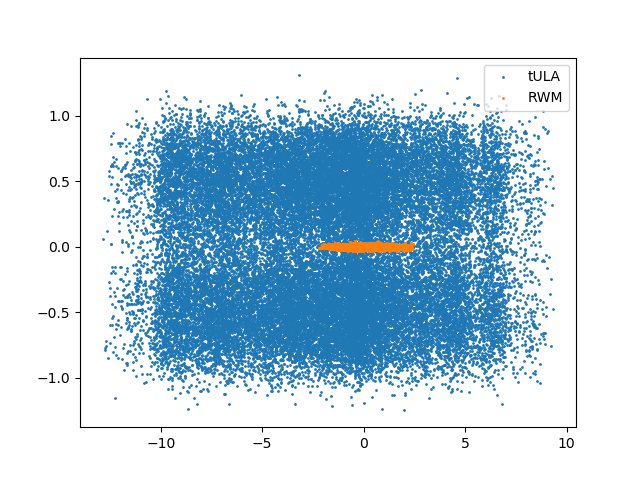
\includegraphics[width=0.8\linewidth]{Figures/transparentTULA.png}
\end{figure}
\end{frame}

\begin{frame}{\texttt{tULAc}     \footnote{Brosse, Durmus, Moulines, Sabanis, 2018}}
    Idea: Use more robust, coordinate-wise, taming!
        \[ X_{n+1} = X_n -hT(X_n) +\sqrt{2h}Z_{n+1} \] \[\]
        \[T=\left(\frac{\partial_i U}{1+h|\partial_i U|}\right)_{i=\lbrace 1, \dots, d\rbrace}\]
   \[\]
   \[\]
   \centerline{\textbf{works well, for small step sizes}}
\end{frame}

\begin{frame}
\begin{figure}
    \centering
    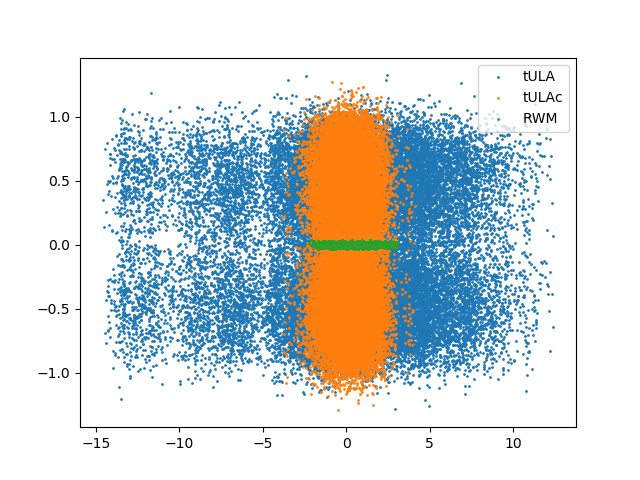
\includegraphics[width=0.8\linewidth]{Figures/transparentBoth.png}
\end{figure}
\end{frame}


\begin{frame}{\texttt{(t)MALA(c)} (\textbf{Metropolis-Adjusted} Langevin Algorithm)    \footnote{Roberts \& Tweedie, 1996}}
    Idea: Use \textbf{Metropolis Hastings}! Gets rid of $\mathcal O (h)$ error.
    
        Make a proposal:
        \[ Y_{n+1} = X_n - h\grad U(X_n)  + \sqrt{2h}Z_{n+1}\] \[\]
        \[ X_{n+1} = \begin{cases}
            Y_{n+1} & \text{ with probability } \alpha = \min \left\lbrace 1, \frac{ \pi\left( Y_{n+1}\right) q (X_n\ |\ Y_{n+1}) } { \pi\left( X_n\right) q (Y_{n+1}\ |\ X_n) } \right\rbrace & \textbf{ ACCEPT } \\ \\ 
            X_n & \text{ otherwise } & \textbf{ REJECT }
        \end{cases}\]
   \[\]
   \[\]
   \centerline{\textbf{problems with acceptance rate}}
\end{frame}


\begin{frame}{\texttt{RWM} \footnote{Metropolis et al. 1953}}
    \textbf{Back to basics}.
    
        Make a proposal:
        \[ Y_{n+1} = X_n + \sqrt{2h}Z_{n+1}\] \[\]
        \[ X_{n+1} = \begin{cases}
            Y_{n+1} & \text{ with probability } \alpha = \min \left\lbrace 1, \frac{ \pi\left( Y_{n+1}\right) } { \pi\left( X_n\right) } \right\rbrace & \textbf{ ACCEPT } \\ \\ 
            X_n & \text{ otherwise } & \textbf{ REJECT }
        \end{cases}\]
   \[\]
   \[\]
   \centerline{\textbf{slow convergence}}
\end{frame}



\begin{frame}
\begin{figure}
    \centering
    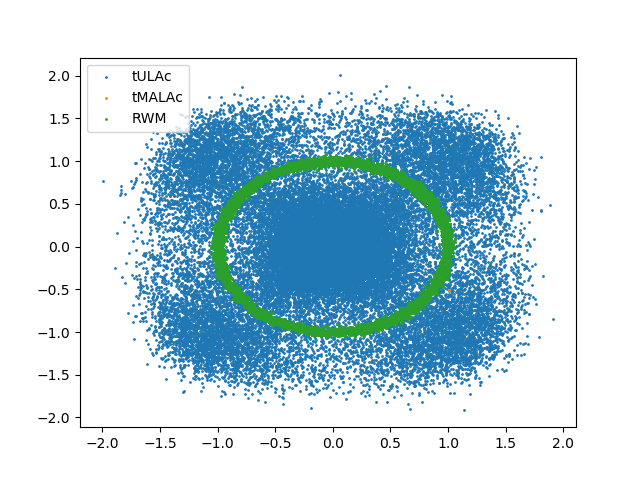
\includegraphics[width=0.8\linewidth]{Figures/transparentDoubleWell.png}
\end{figure}
\end{frame}


% \begin{frame}{Horse Racing? Us vs. Brosse et al.}
%     Show off our numeric skills
    
%     Brosse et al. - `Given the results of the numerical experiments, TULAc should be chosen over ULA
% to sample from general probability distributions. Indeed, TULAc has similar results as
% ULA when the step size is small and is more stable when using larger step sizes.'
% \end{frame}

\begin{frame}{Which algorithm to use?}
    \begin{itemize}
        \item Highly dependent on application.
        \item Trade-off between quality and feasible speed.
        \item Other approaches:
        \begin{itemize}
            \item Higher order schemes (\texttt{HOLA})
            \item \texttt{HMC}, \texttt{mMALA}, \texttt{SGLD} (Stochastic Gradient Langevin Dynamics)
        \end{itemize}
    \end{itemize}

    % What algorithm is best in what situation?
    % Next Steps:\\
    % Test use on real data, parallelise algs with complex iterations (HOLA), compare with some ML tech?
    \end{frame}

% \begin{frame}{Future Work}
% There are many many methods we haven't considered: SGLD, HMC, mMALA。 \\
% \end{frame}

\begin{frame}{Why \texttt{SGLD}?}
  \begin{itemize}
      \item Normally, samples in machine learning are of huge sample sizes, for which most MCMC algorithms are not designed to process. 
      \item Stochastic Gradient Langevin Dynamics (\texttt{SGLD}) is a popular one. 
      \item \texttt{SGLD} is based on the Langevin Monte Carlo.\\
            It uses unbiased estimator of the gradient of log-posterior based on subsampling, suitable for samples of huge size. 
  \end{itemize} 
\end{frame}
\begin{frame}{\texttt{SGLD}}
\begin{itemize}
    \item $\nabla U \to \nabla U_0+(\frac{N}{p}) \sum_{i\in S}\nabla U_i$,  where S is a minibatch of \{1,...., N\} with replacement of size p.\\
    N is the size of the sample, p is the size of the subsample. 
    $U_0$ is log-prior, $U_i$ is log-likelihood.
\item Our iterations:
$$X_{n+1} = X_{n}-h \Bigg (\nabla U_0(X_n)+\frac{N}{p}\sum_{i\in S_{n+1}}\nabla U_i(X_n)\Bigg )+\sqrt{2h}Z_{n+1}$$

$h > 0$: constant step size & $(Z_n)_{n\geq1}$: a sequence of i.i.d standard d - dimensional Gaussian vectors. 
\end{itemize}
\end{frame}
\begin{frame}{\texttt{SGD}}
    Stochastic Gradient Descent (SGD) is SGLD without the Gaussian noise, (the last term):

$$X_{n+1} = X_{n}-h \Bigg (\nabla U_0(X_n)+\frac{N}{p}\sum_{i\in S_{n+1}}\nabla U_i(X_n)\Bigg)$$

SGLD is similar to SGD, a well-known algorithm for optimization. 
\end{frame}




\begin{frame}{Future Work}
\begin{itemize}
    \item To test these methods on  real or simulated data when we don't know the gradient analytically.
   \item In higher dimension, taming methods may be better than the others.
    \item In higher dimension, for sample of large size, we will use SGLD algorithms to reduce the costs.
\end{itemize}
\end{frame}



\begin{frame}{\textsc{Python} implementation }
    We have implemented a suite of tools for analysis of the above LMC algorithms. 
    
    \begin{figure}
    \centering
    
\includegraphics[width=0.8\linewidth]{Figures/cloud.png}
    \end{figure}
    
    \textbf{\centerline{\url{https://github.com/Tom271/LangevinMC}}}
\end{frame}

% \begin{frame}{First and Second Moments of Double Well - \(h=0.01\)}%{Optional Subtitle}
%         \begin{figure}[h]
%         \centering
%         \begin{minipage}{0.5\linewidth}
%           \centering
%           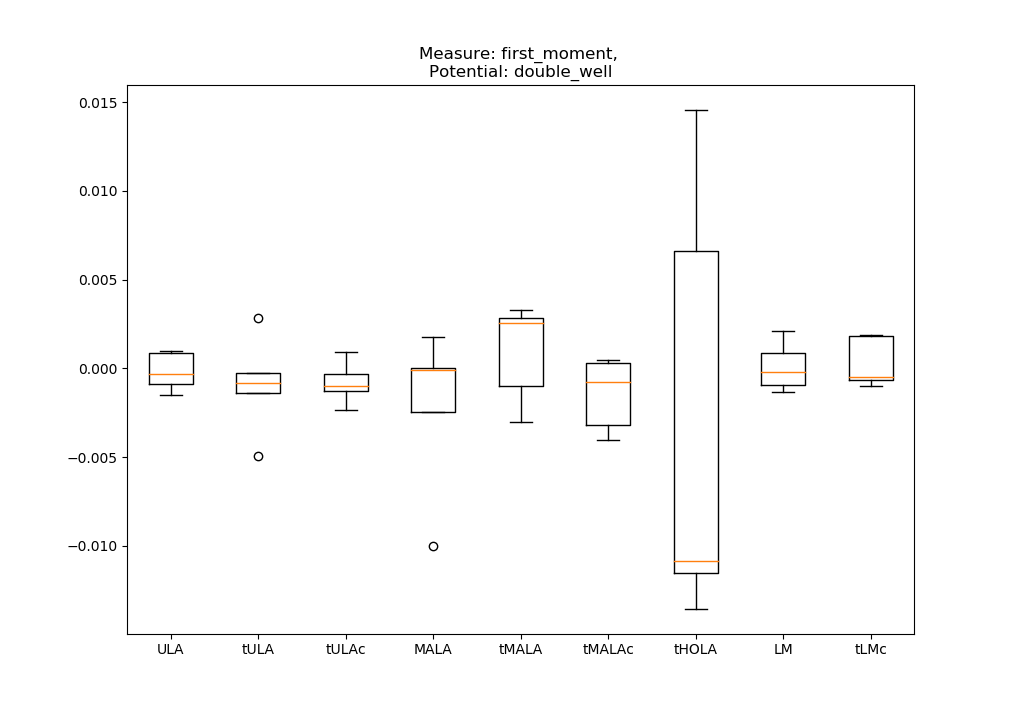
\includegraphics[width=0.99\linewidth]{10sBoxPlot1moment100dim001step.png}
%         \end{minipage}%
%         \begin{minipage}{0.5\linewidth}
%           \centering
%           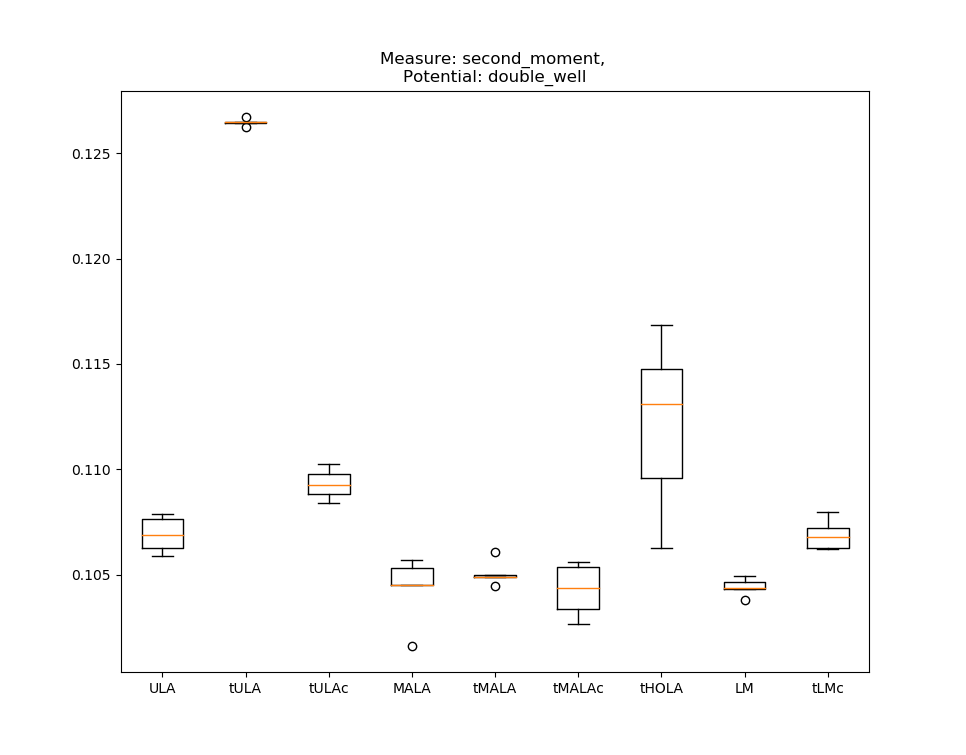
\includegraphics[width=0.99\linewidth]{10sBoxPlot2moment100dim001step.png}
%         \end{minipage}%
%         \end{figure}
% \end{frame}

% \begin{frame}{First and Second Moments of Double Well - \(h=0.1\)}%{Optional Subtitle}
%         \begin{figure}[h]
%         \centering
%         \begin{minipage}{0.5\linewidth}
%           \centering
%           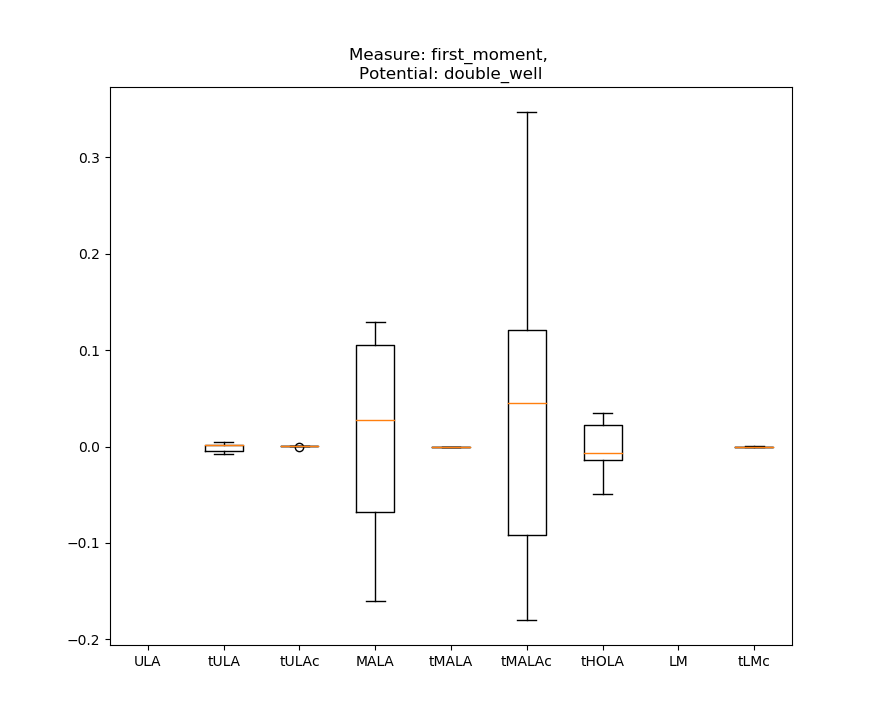
\includegraphics[width=0.99\linewidth]{10sBoxPlot1moment100dim01step.png}
%         \end{minipage}%
%         \begin{minipage}{0.5\linewidth}
%           \centering
%           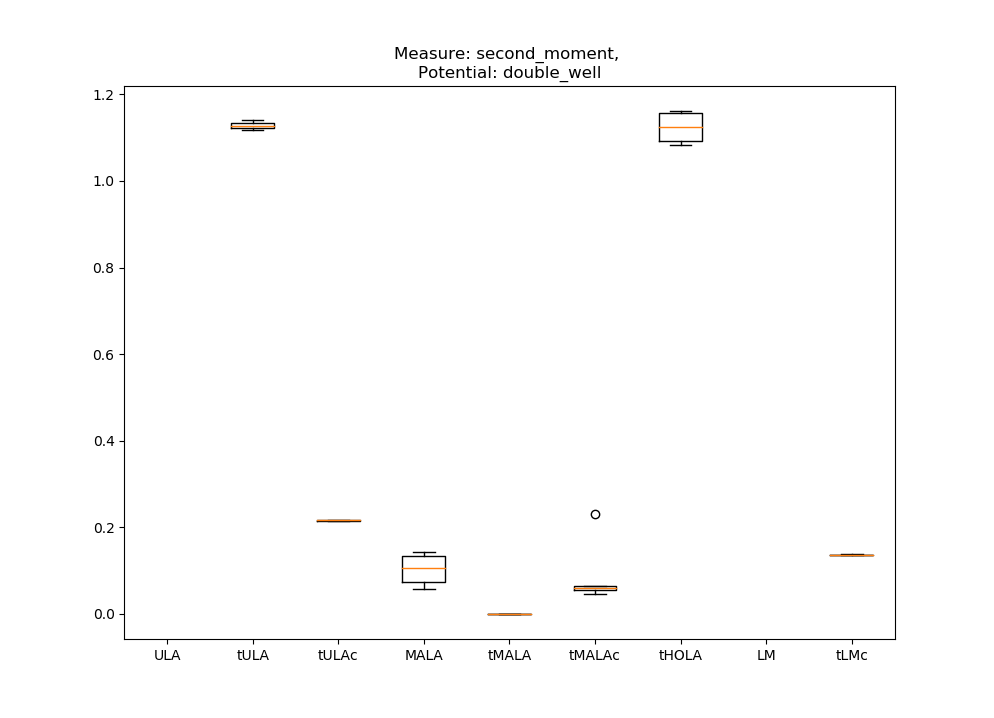
\includegraphics[width=0.99\linewidth]{10sBoxPlot2moment100dim01step.png}
%         \end{minipage}%
%         \end{figure}
% \end{frame}



% \begin{frame}{First and Second Moments of Ill-Condition Gaussian - 1st Dimension}%{Optional Subtitle}
%         \begin{figure}[h]
%         \centering
%         \begin{minipage}{0.5\linewidth}
%           \centering
%           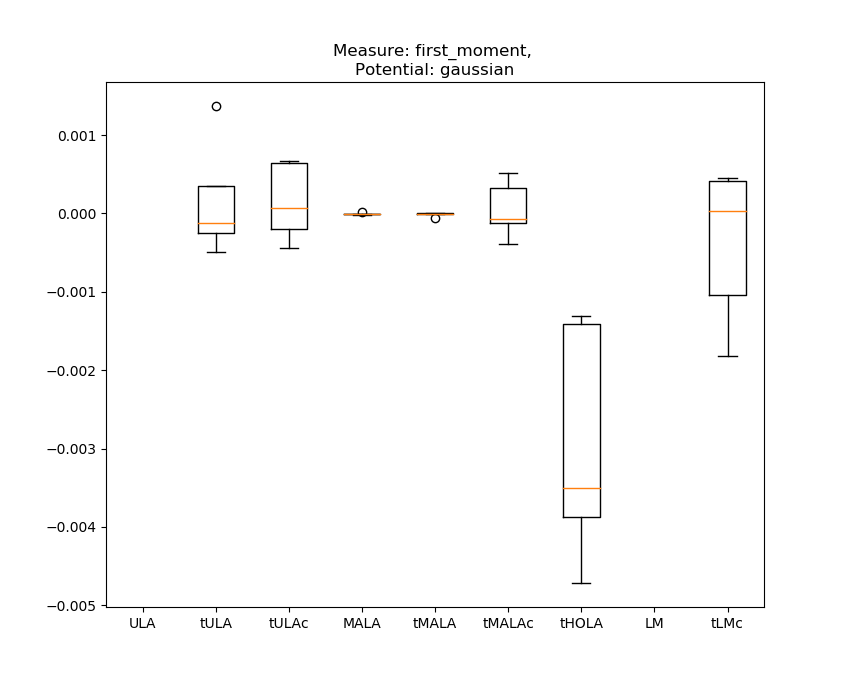
\includegraphics[width=0.99\linewidth]{illcond10sBoxPlot1moment100dim01step.png}
%         \end{minipage}%
%         \begin{minipage}{0.5\linewidth}
%           \centering
%           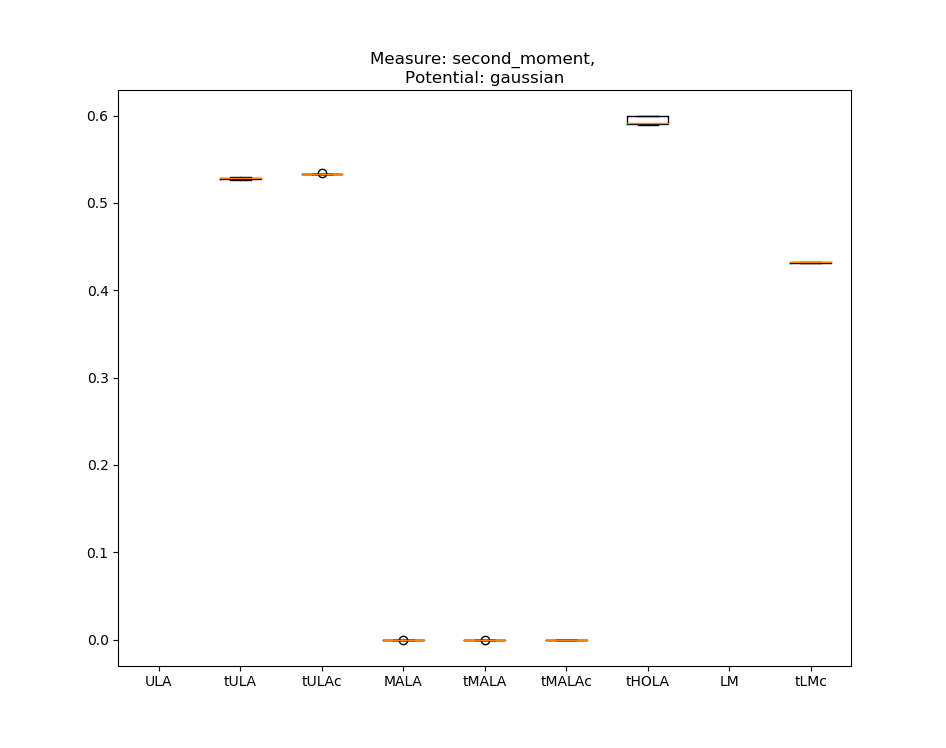
\includegraphics[width=0.99\linewidth]{illcond10sBoxPlot2moment100dim01step.png}
%         \end{minipage}%
%         \end{figure}
% \end{frame}

% \begin{frame}{First and Second Moments of Ill-Condition Gaussian - 2nd Dimension}%{Optional Subtitle}
%         \begin{figure}[h]
%         \centering
%         \begin{minipage}{0.5\linewidth}
%           \centering
%           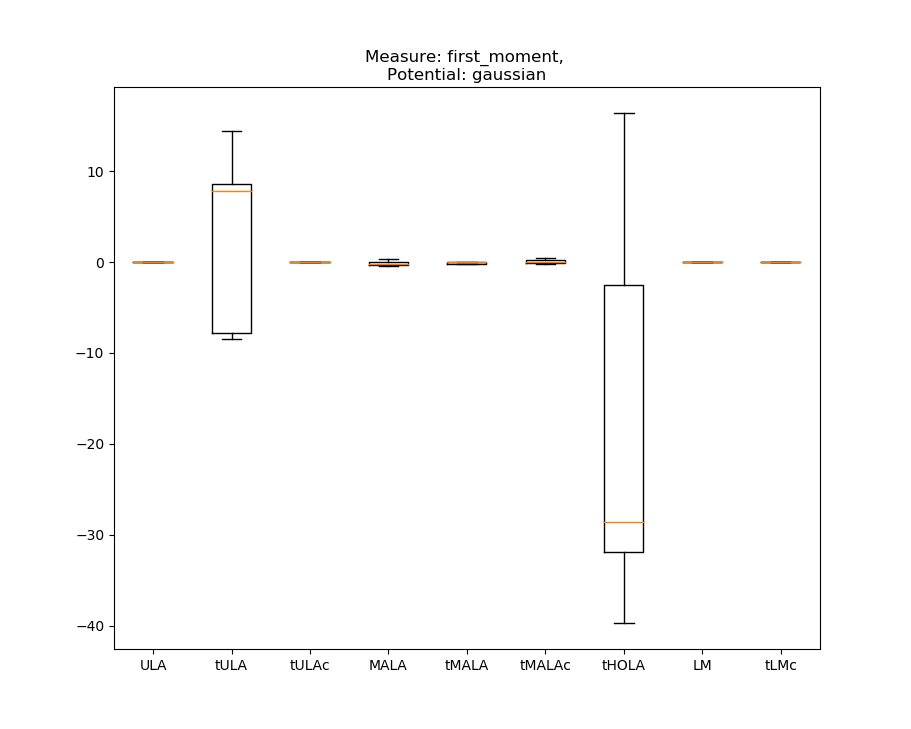
\includegraphics[width=0.99\linewidth]{illcond10sBoxPlot1moment100dim01step2nddim.png}
%         \end{minipage}%
%         \begin{minipage}{0.5\linewidth}
%           \centering
%           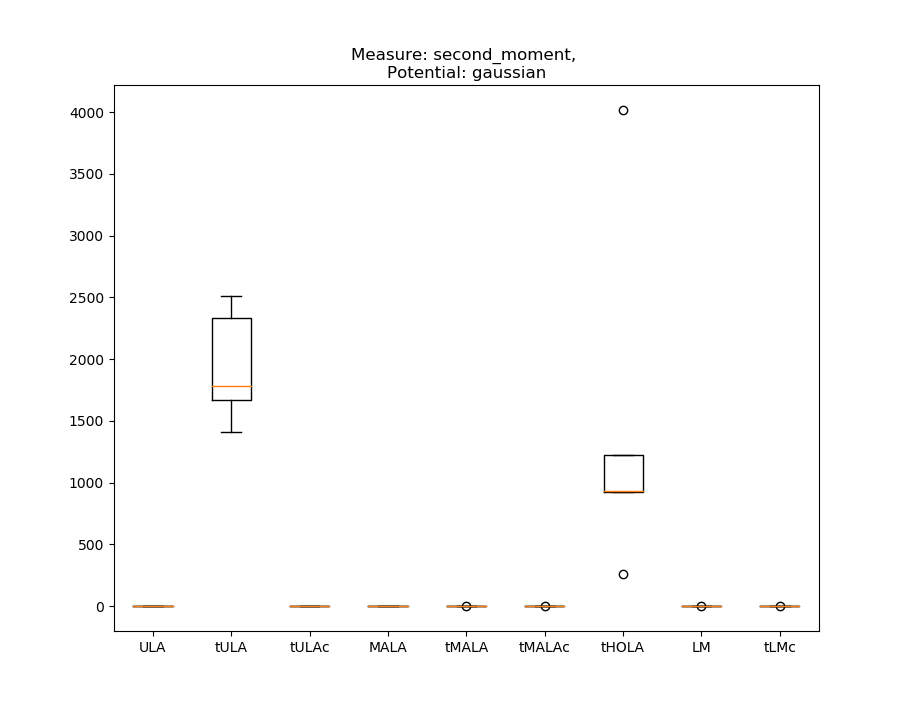
\includegraphics[width=0.99\linewidth]{illcond10sBoxPlot2moment100dim01step2nddim.png}
%         \end{minipage}%
%         \end{figure}
% \end{frame}
% \begin{frame}{First and Second Moments of Ill-Condition Gaussian - 2nd Dimension}%{Optional Subtitle}
%         \begin{figure}[h]
%         \centering
%         \begin{minipage}{0.7\linewidth}
%           \centering
%           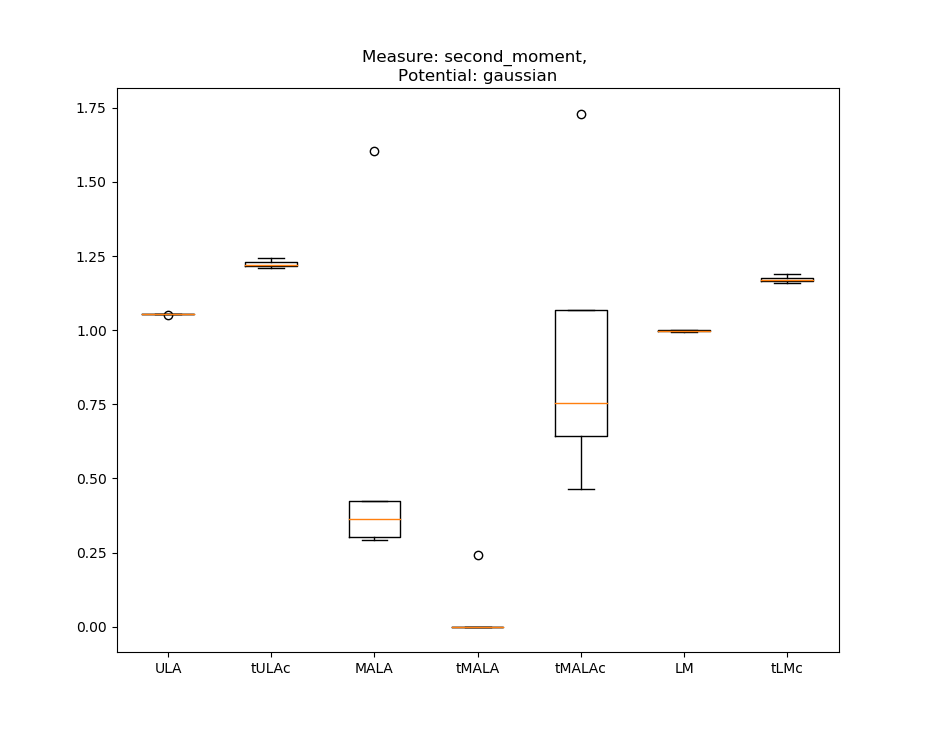
\includegraphics[width=0.99\linewidth]{illcond10sBoxPlot2moment100dim01step2nddimnotula.png}
%         \end{minipage}%
%         \end{figure}
% \end{frame}



% \subsection{Non-asymptotic behaviour}
% \begin{frame}{Beyond Moments}
% \begin{itemize}
%     \item Total Variation
%         \[\|\mu-\nu\|_{TV} - \sup_{\|f\|\leq 1} |\mu(f) - \nu(f)|\ \]
%     \item Wasserstein Distance
%       \[W_2(\mu,\nu) = \left( \inf_{\gamma \in \Gamma(\mu,\nu)} \int_{M\times M} d(x,y)^2 \mathrm{d}\gamma(x,y)\right)^{\frac{1}{2}}\]
% \end{itemize}

% \end{frame}

% \begin{frame}{Durmus--Moulines Bounds}
% \begin{figure}[h]
%     \centering
%     \begin{subfigure}[b]{\textwidth}
%         \centering
%         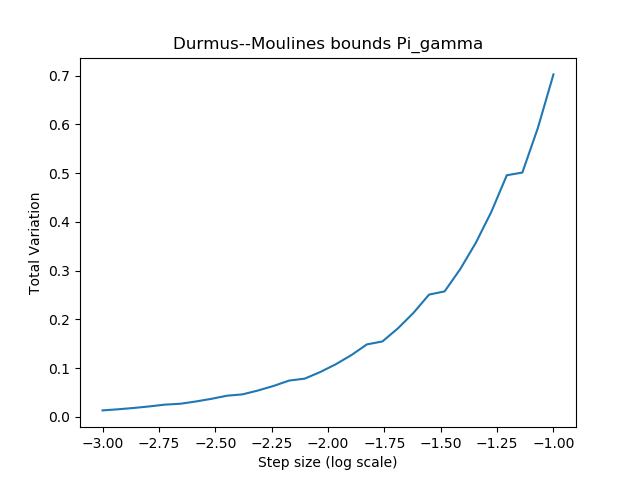
\includegraphics[width=0.23\textwidth]{Pi_gamma.png}
%         \caption{Error in $\pi_\gamma$ (Choose suitable step size)}
%     \end{subfigure}

% \end{figure}
% \begin{figure}[h]
%     \centering
%     \begin{subfigure}[b]{0.23\textwidth}
%         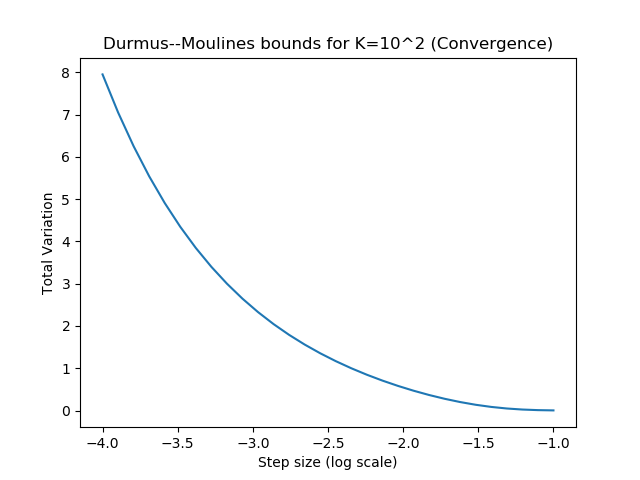
\includegraphics[width=\textwidth]{ConvergenceK1e2.png}
%         \caption{K=$10^2$}
%     \end{subfigure}
%     ~ %add desired spacing between images, e. g. ~, \quad, \qquad, \hfill etc. 
%       %(or a blank line to force the subfigure onto a new line)
%     \begin{subfigure}[b]{0.23\textwidth}
%         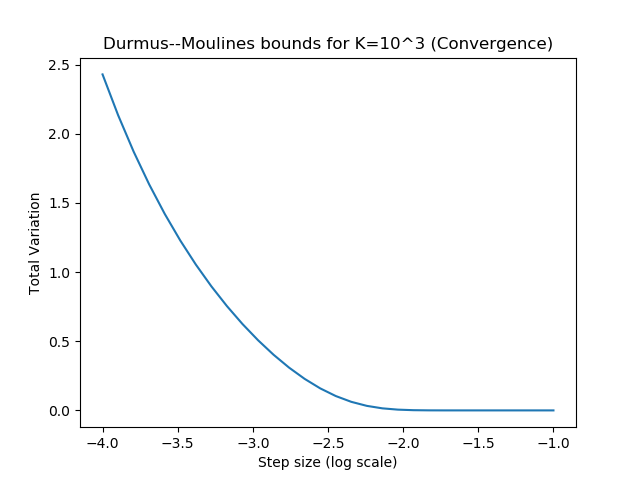
\includegraphics[width=\textwidth]{ConvergenceK1e3.png}
%         \caption{K=$10^3$}
%     \end{subfigure}
%     ~ %add desired spacing between images, e. g. ~, \quad, \qquad, \hfill etc. 
%     %(or a blank line to force the subfigure onto a new line)
%     \begin{subfigure}[b]{0.23\textwidth}
%         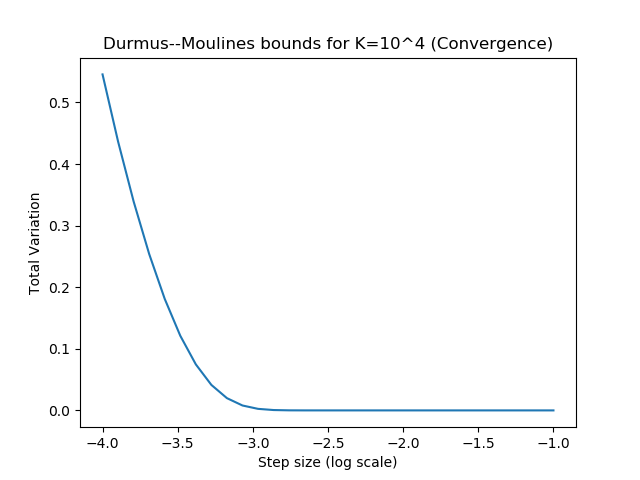
\includegraphics[width=\textwidth]{ConvergenceK1e4.png}
%         \caption{K=$10^4$}
%     \end{subfigure}
%     ~
%     \begin{subfigure}[b]{0.23\textwidth}
%         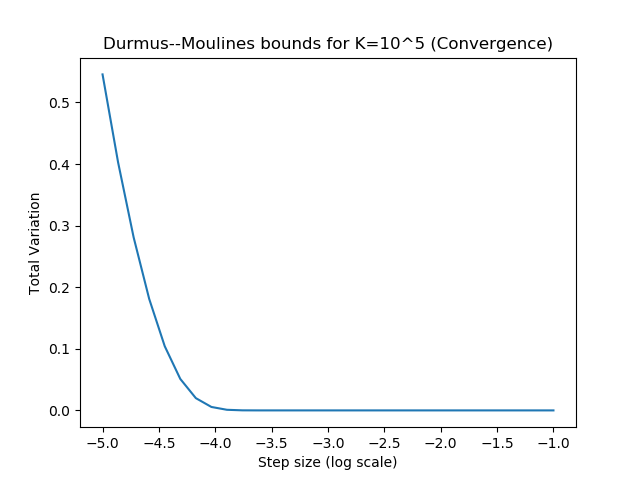
\includegraphics[width=\textwidth]{ConvergenceK1e5.png}
%         \caption{K=$10^5$}
%     \end{subfigure}
    
% \end{figure}
% \end{frame}

% \subsection{Future}

% \begin{frame}{Future Work}
% \begin{itemize}
%     \item Check Dalalyan's new `user-friendly' bound
%     \item Are these bounds anywhere near sharp?
%     \item Test against SGLD
%     \item Test on real data
% \end{itemize}
    
% \end{frame}






% You can reveal the parts of a slide one at a time
% with the \pause command:
% \begin{frame}{Second Slide Title}
%   \begin{itemize}
%   \item {
%     First item.
%     \pause % The slide will pause after showing the first item
%   }
%   \item {   
%     Second item.
%   }
%   % You can also specify when the content should appear
%   % by using <n->:
%   \item<3-> {
%     Third item.
%   }
%   \item<4-> {
%     Fourth item.
%   }

%   % or you can use the \uncover command to reveal general
%   % content (not just \items):
%   \item<5-> {
%     Fifth item. \uncover<6->{Extra text in the fifth item.}
%   }
%   \end{itemize}
 % \end{frame}




\end{document}


